\chapter{An Appendix Chapter}
\label{appn:A}

\section{Topic-Wise Acceptance Rates for Each Prompt}
This section presents the topic-wise acceptance rates for each of the nine prompts used in the study. These figures illustrate how the model performed across various computer science topics, highlighting areas of strength and weakness for each prompt. These visualizations serve as a valuable tool for understanding the specific strengths and weaknesses of the AI model in solving diverse coding problems, and it can guide future research and prompt engineering efforts to enhance model performance.

\begin{figure}[H]
    \centering
    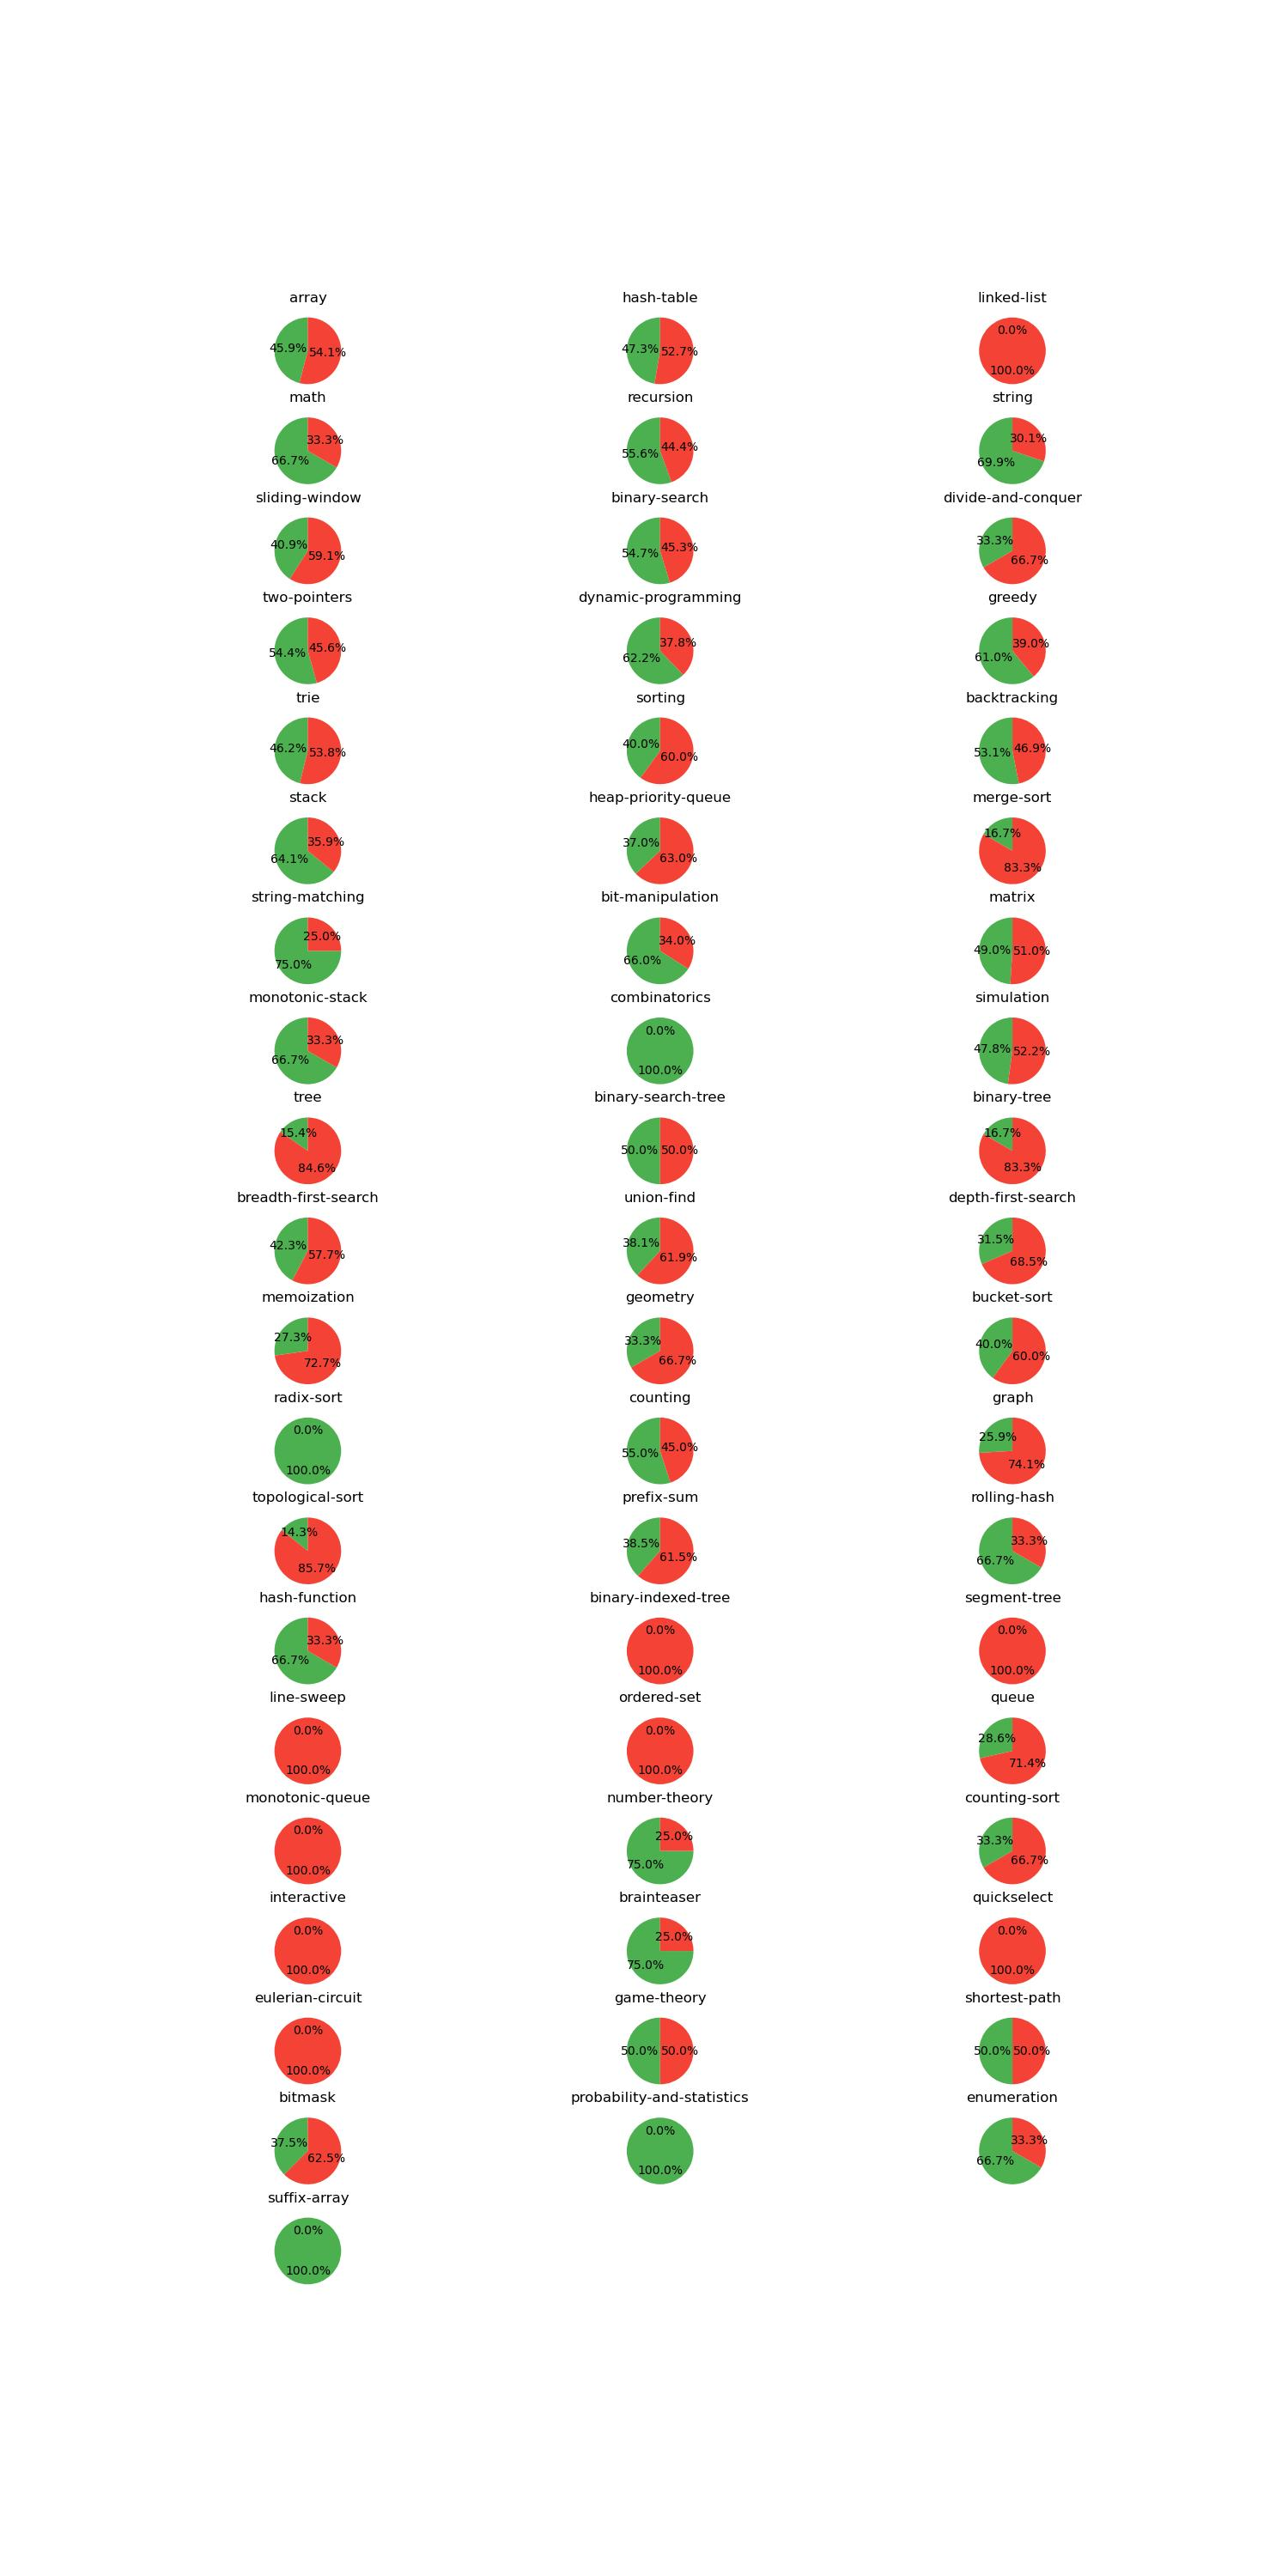
\includegraphics[width=0.75\textwidth, height=0.7\textheight]{figures/1/accepted_not_topicwise.jpg}
    \caption{Topic-wise acceptance rate for Prompt 1, illustrating the percentage of solutions accepted (green) and not accepted (red) across different undergraduate computer science topics.}
    \label{fig:topic_wise_acceptance_prompt_1}
\end{figure}

\begin{figure}[H]
    \centering
    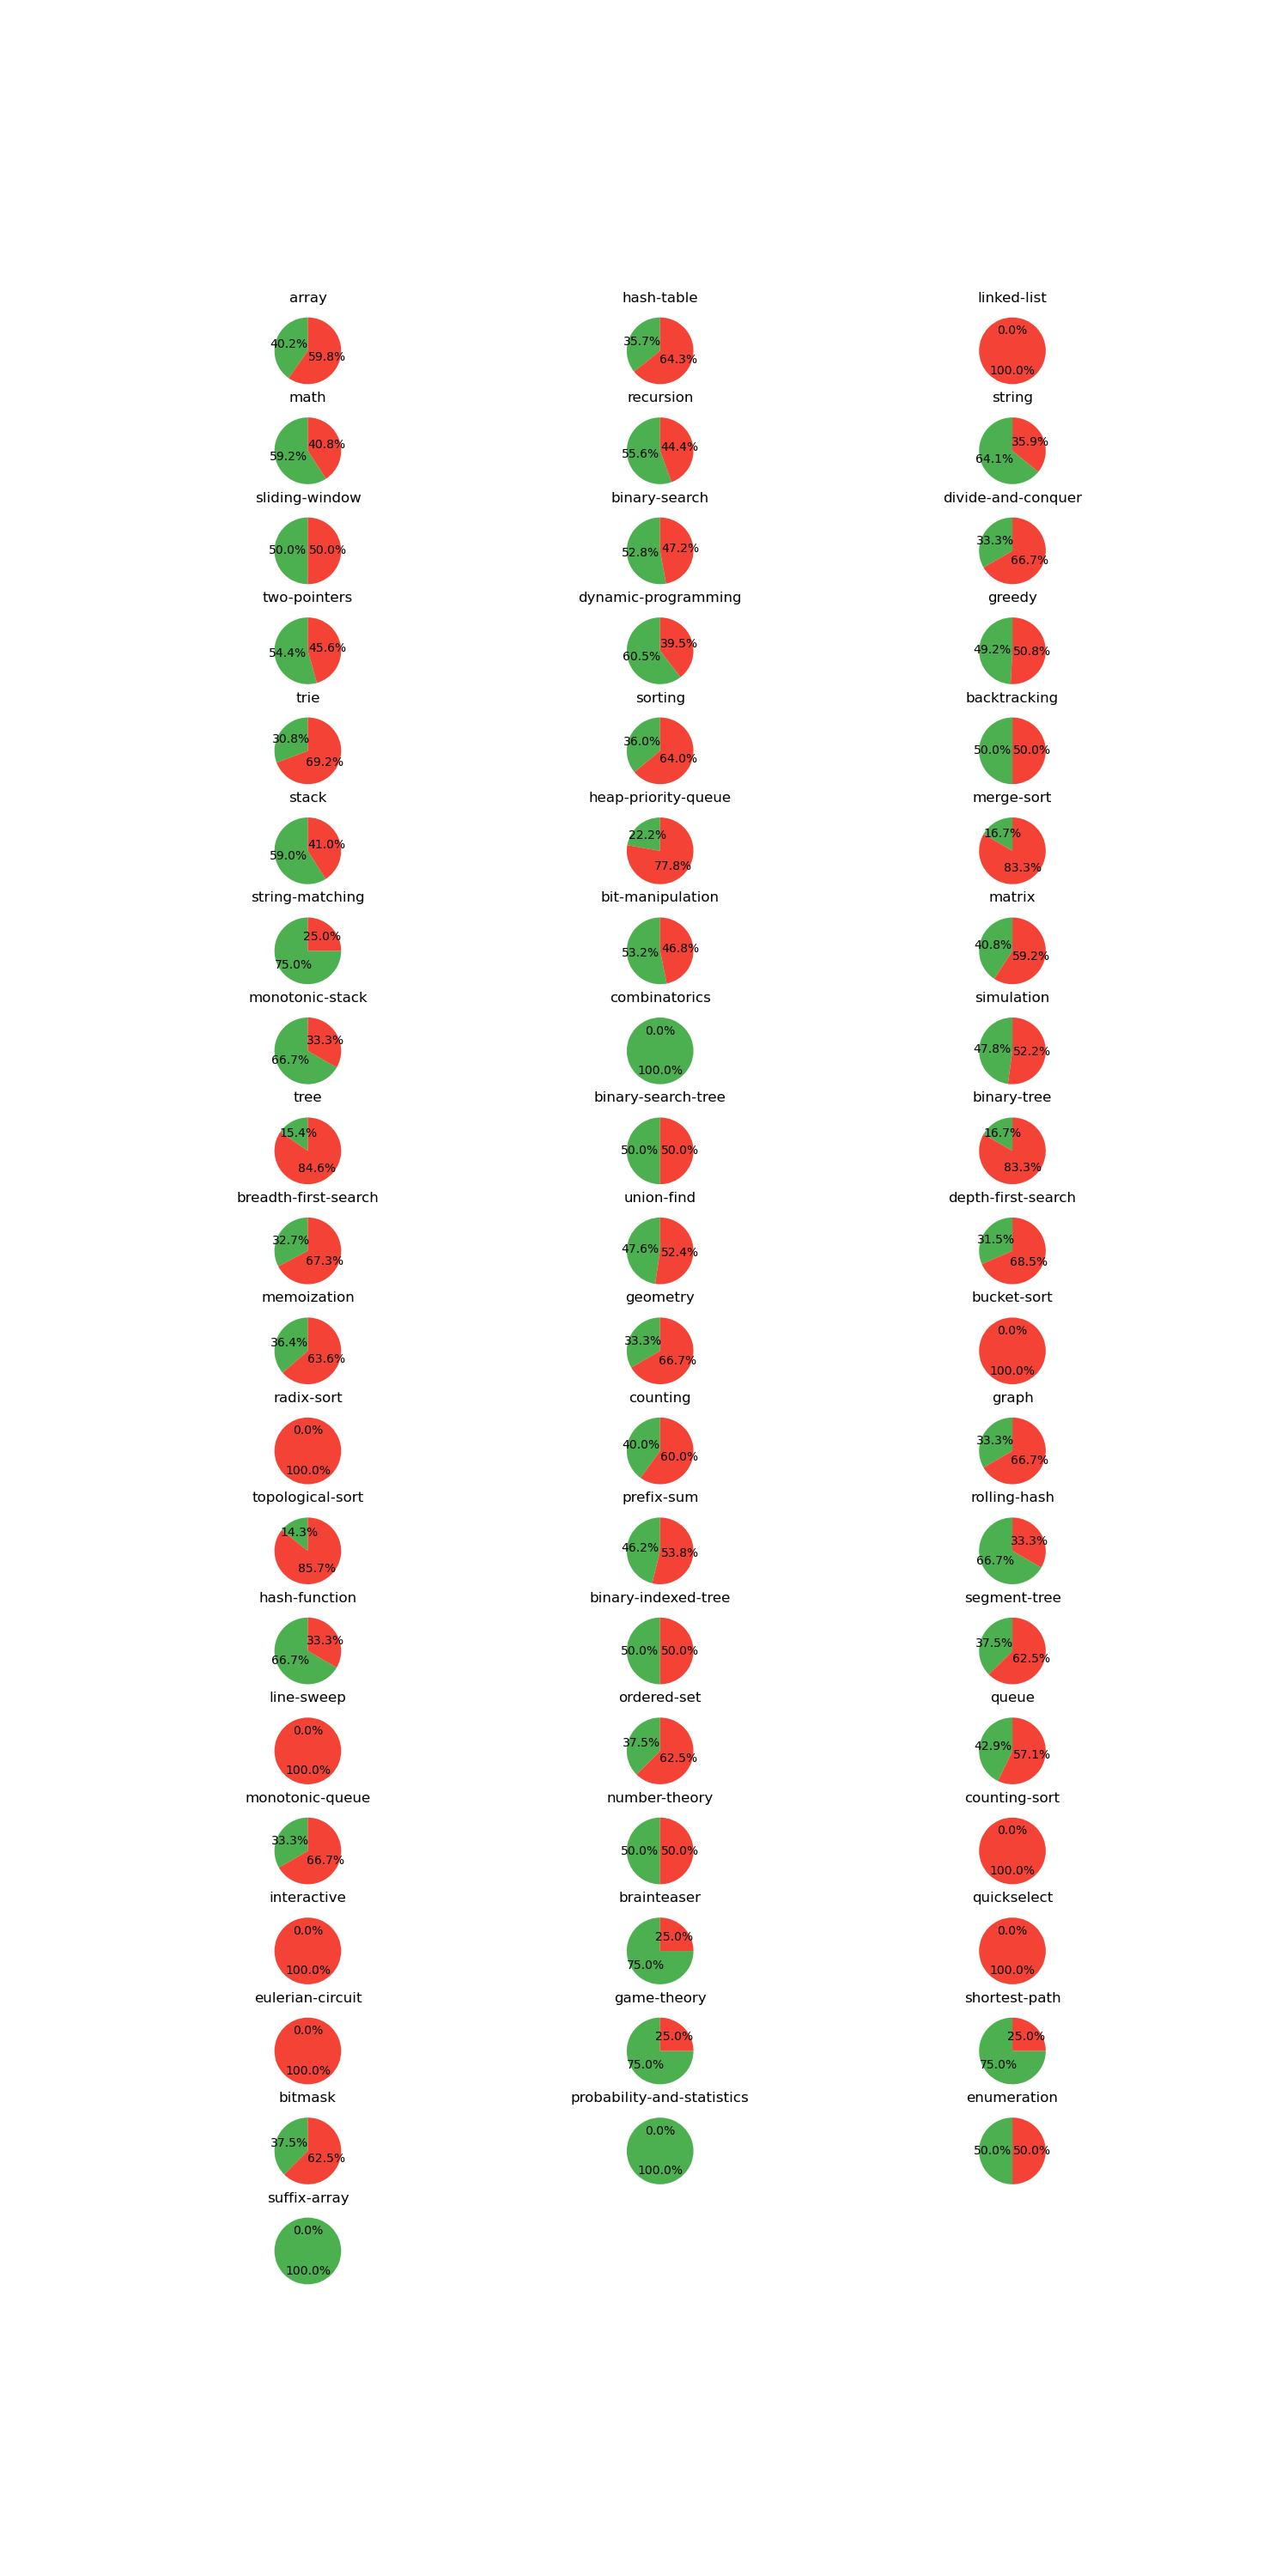
\includegraphics[width=0.75\textwidth, height=0.7\textheight]{figures/2/accepted_not_topicwise.jpg}
    \caption{Topic-wise acceptance rate for Prompt 2, illustrating the percentage of solutions accepted (green) and not accepted (red) across different undergraduate computer science topics.}
    \label{fig:topic_wise_acceptance_prompt_2}
\end{figure}

\begin{figure}[H]
    \centering
    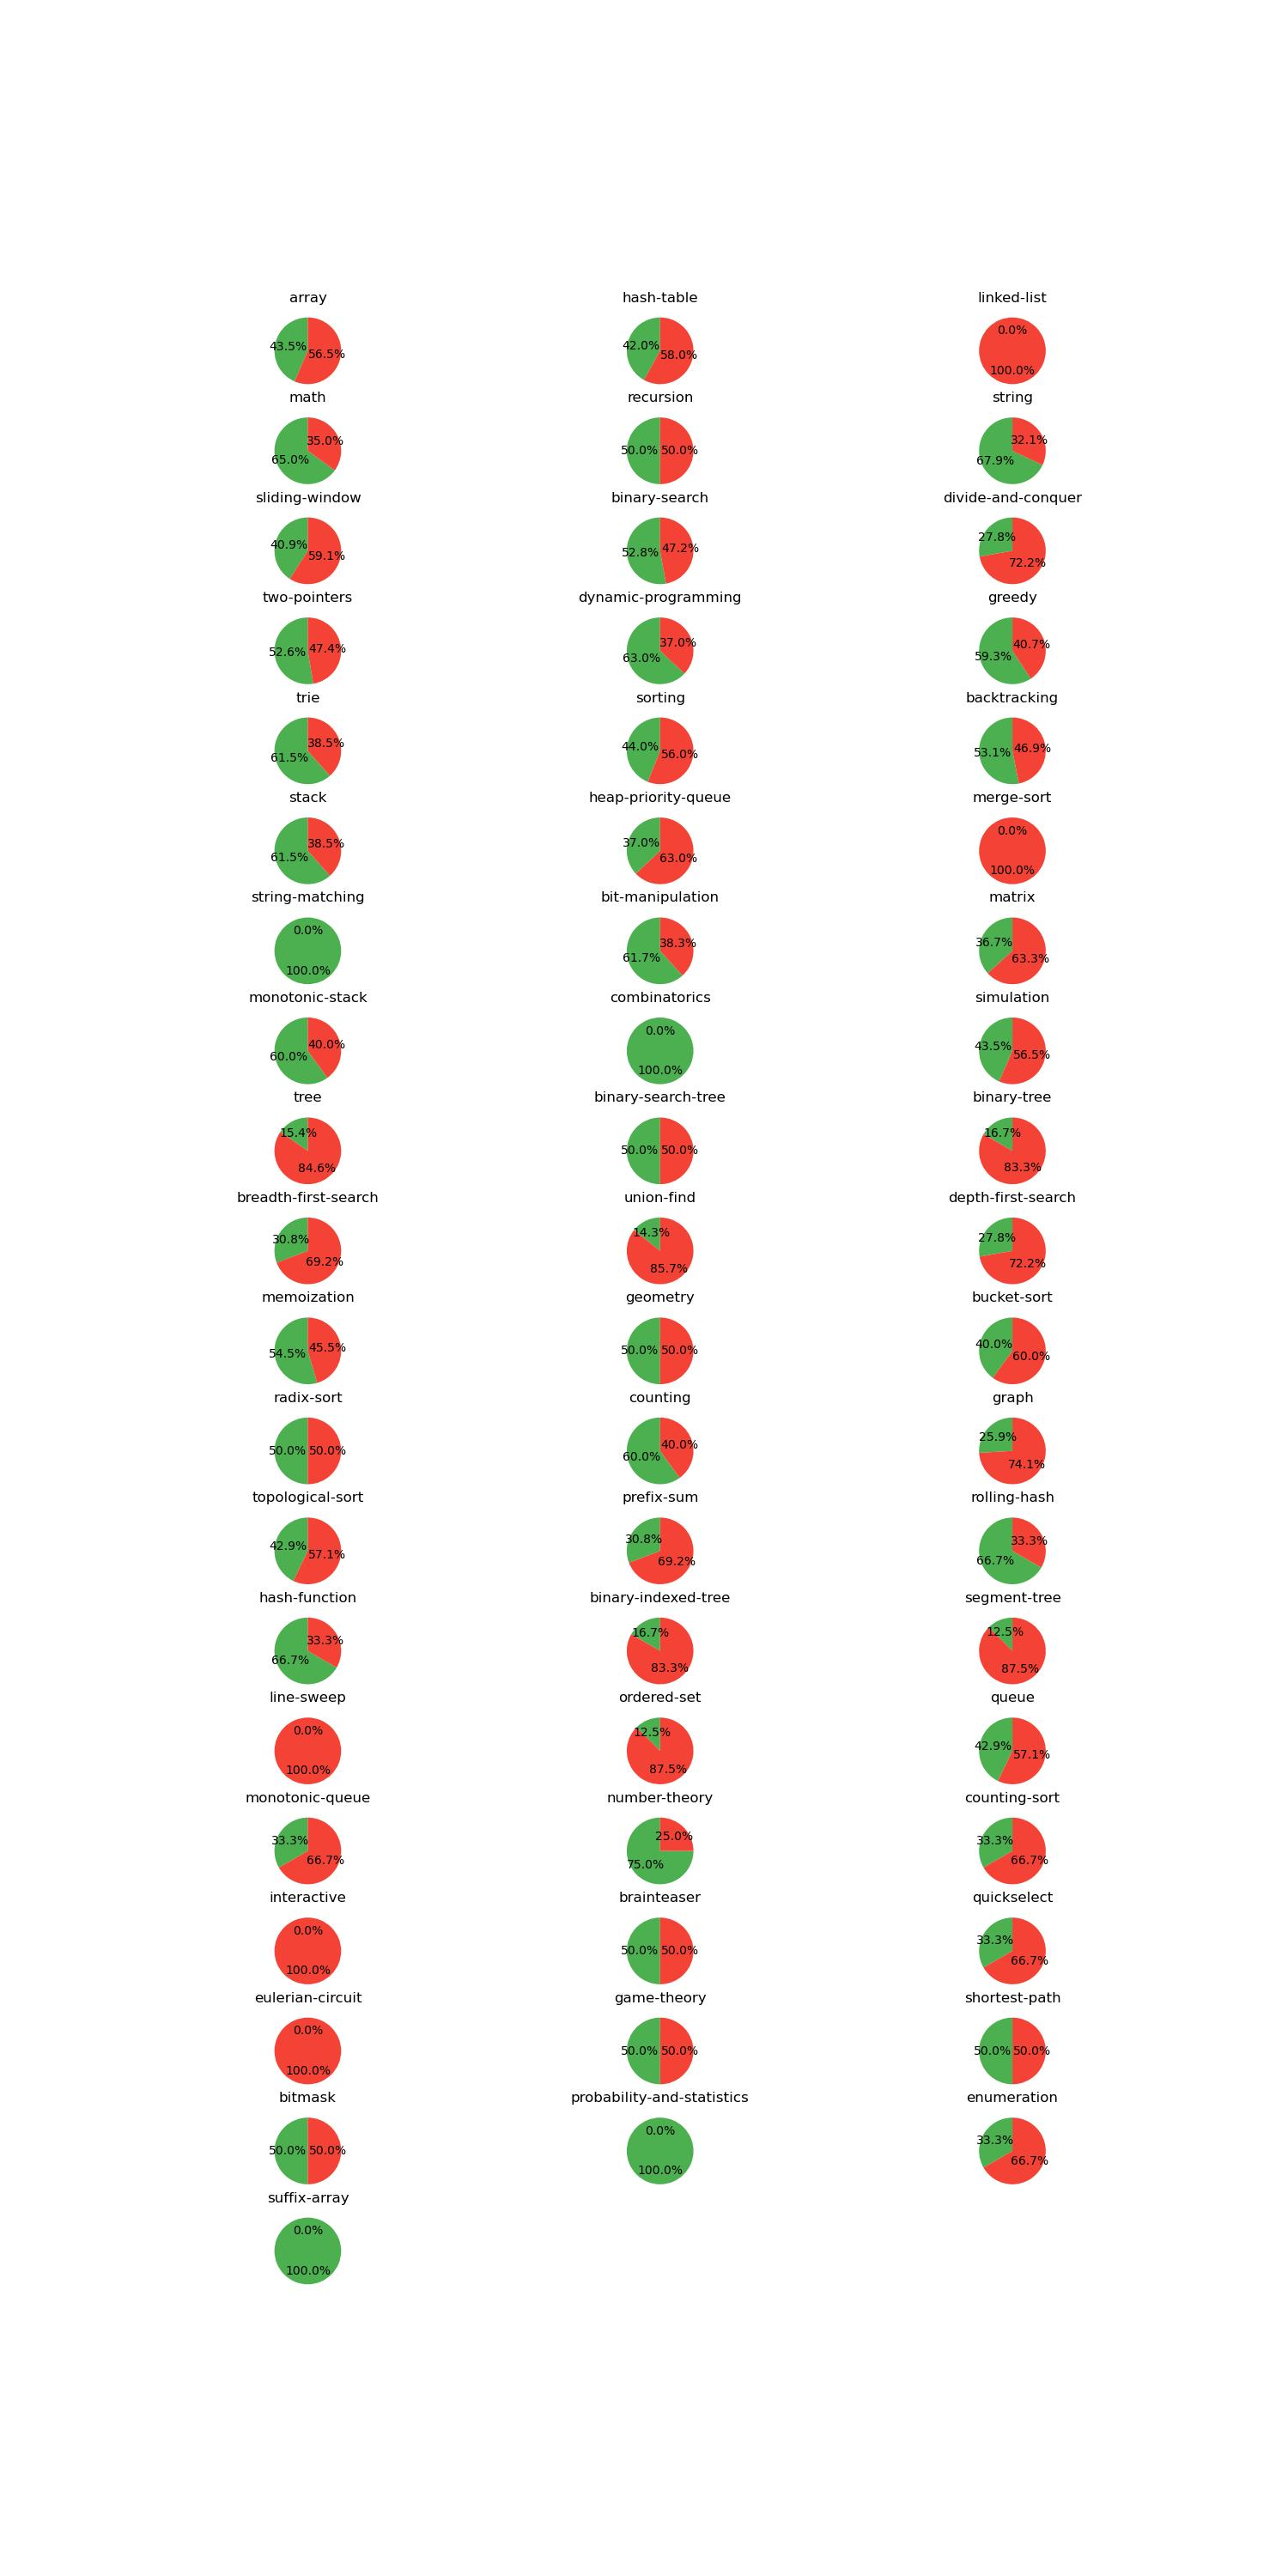
\includegraphics[width=0.75\textwidth, height=0.7\textheight]{figures/3/accepted_not_topicwise.jpg}
    \caption{Topic-wise acceptance rate for Prompt 3, illustrating the percentage of solutions accepted (green) and not accepted (red) across different undergraduate computer science topics.}
    \label{fig:topic_wise_acceptance_prompt_3}
\end{figure}

\begin{figure}[H]
    \centering
    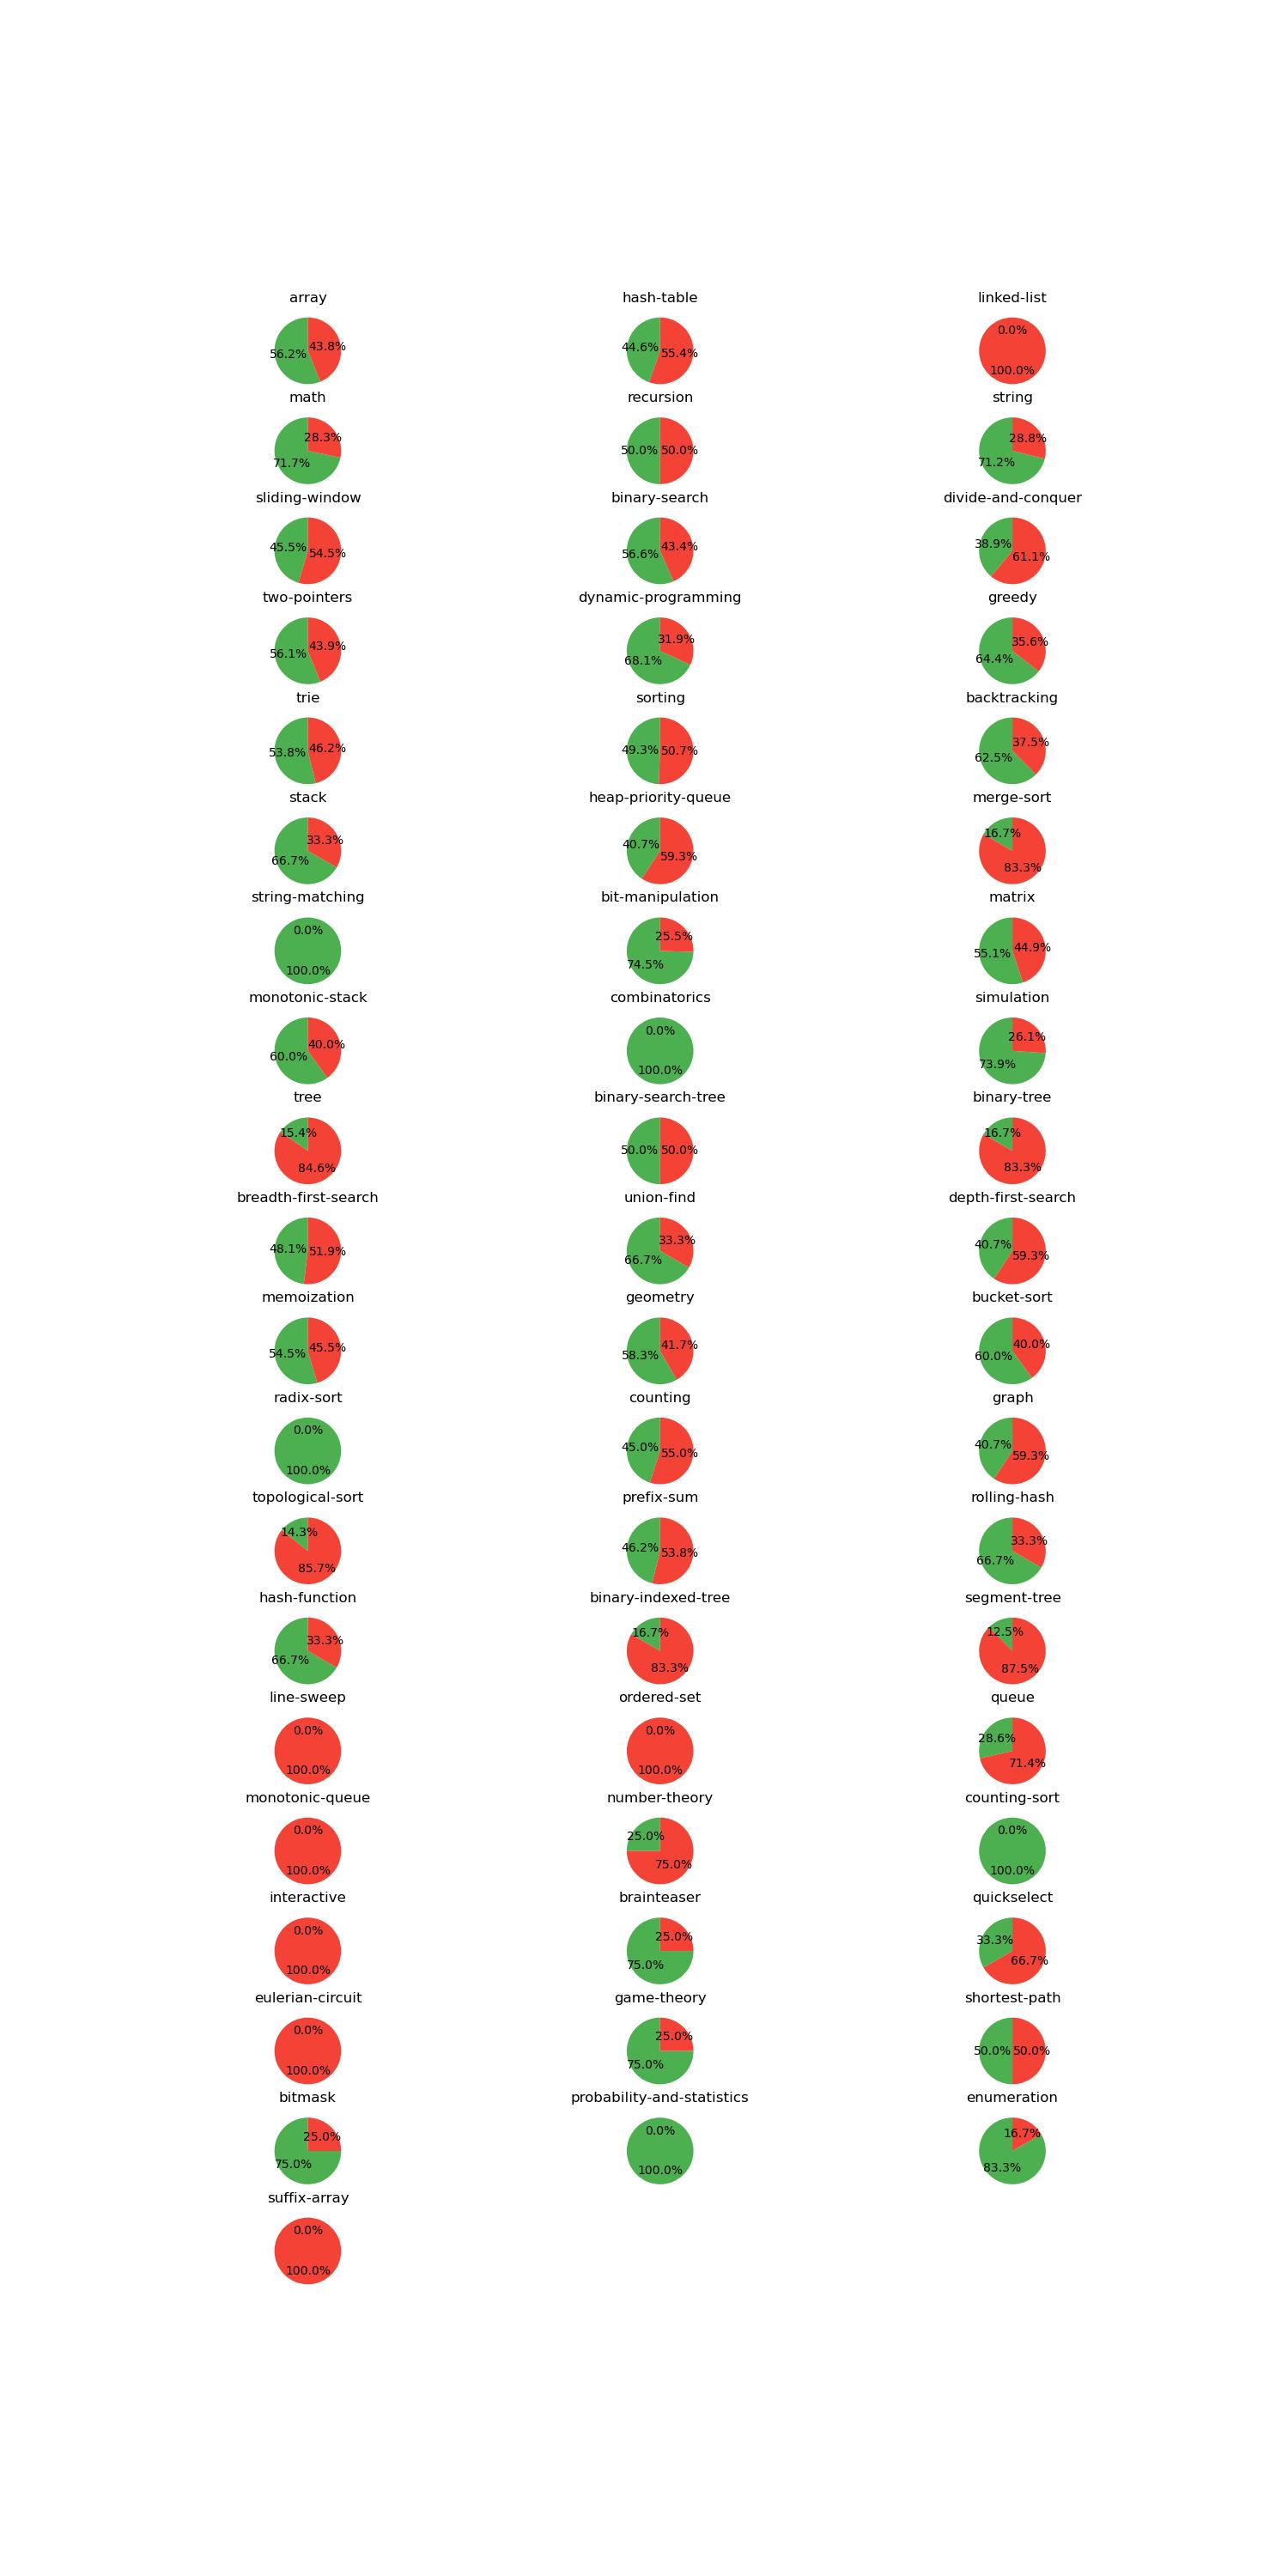
\includegraphics[width=0.75\textwidth, height=0.7\textheight]{figures/4/accepted_not_topicwise.jpg}
    \caption{Topic-wise acceptance rate for Prompt 4, illustrating the percentage of solutions accepted (green) and not accepted (red) across different undergraduate computer science topics.}
    \label{fig:topic_wise_acceptance_prompt_4}
\end{figure}

\begin{figure}[H]
    \centering
    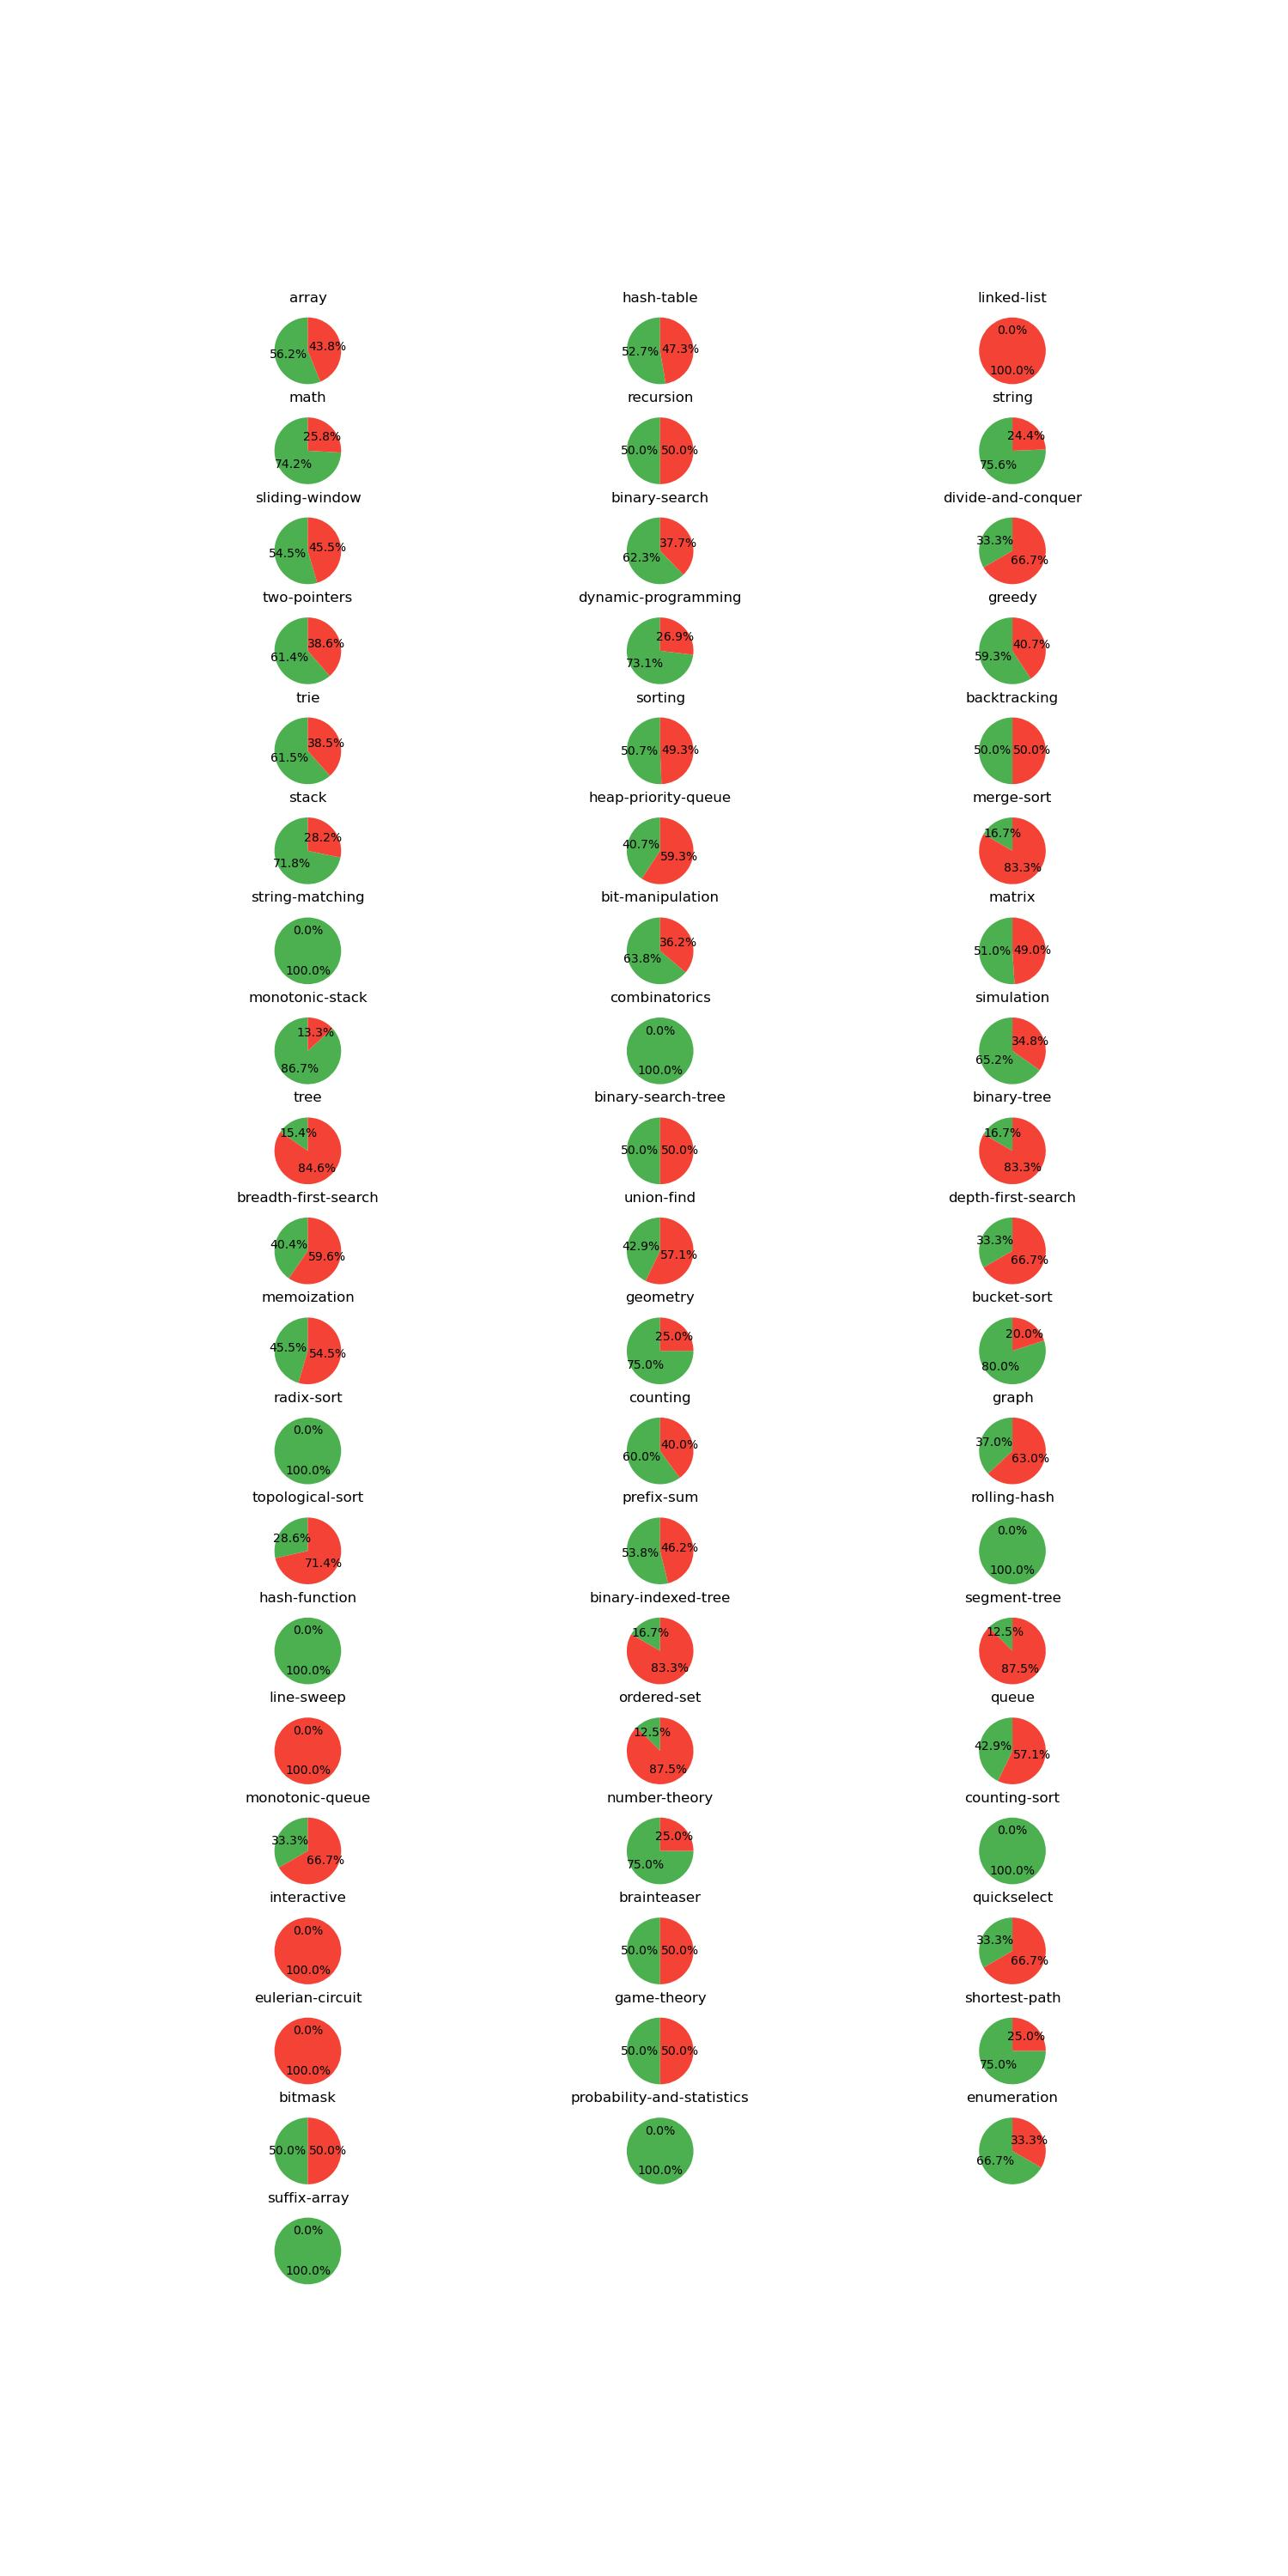
\includegraphics[width=0.75\textwidth, height=0.7\textheight]{figures/5/accepted_not_topicwise.jpg}
    \caption{Topic-wise acceptance rate for Prompt 5, illustrating the percentage of solutions accepted (green) and not accepted (red) across different undergraduate computer science topics.}
    \label{fig:topic_wise_acceptance_prompt_5}
\end{figure}

\begin{figure}[H]
    \centering
    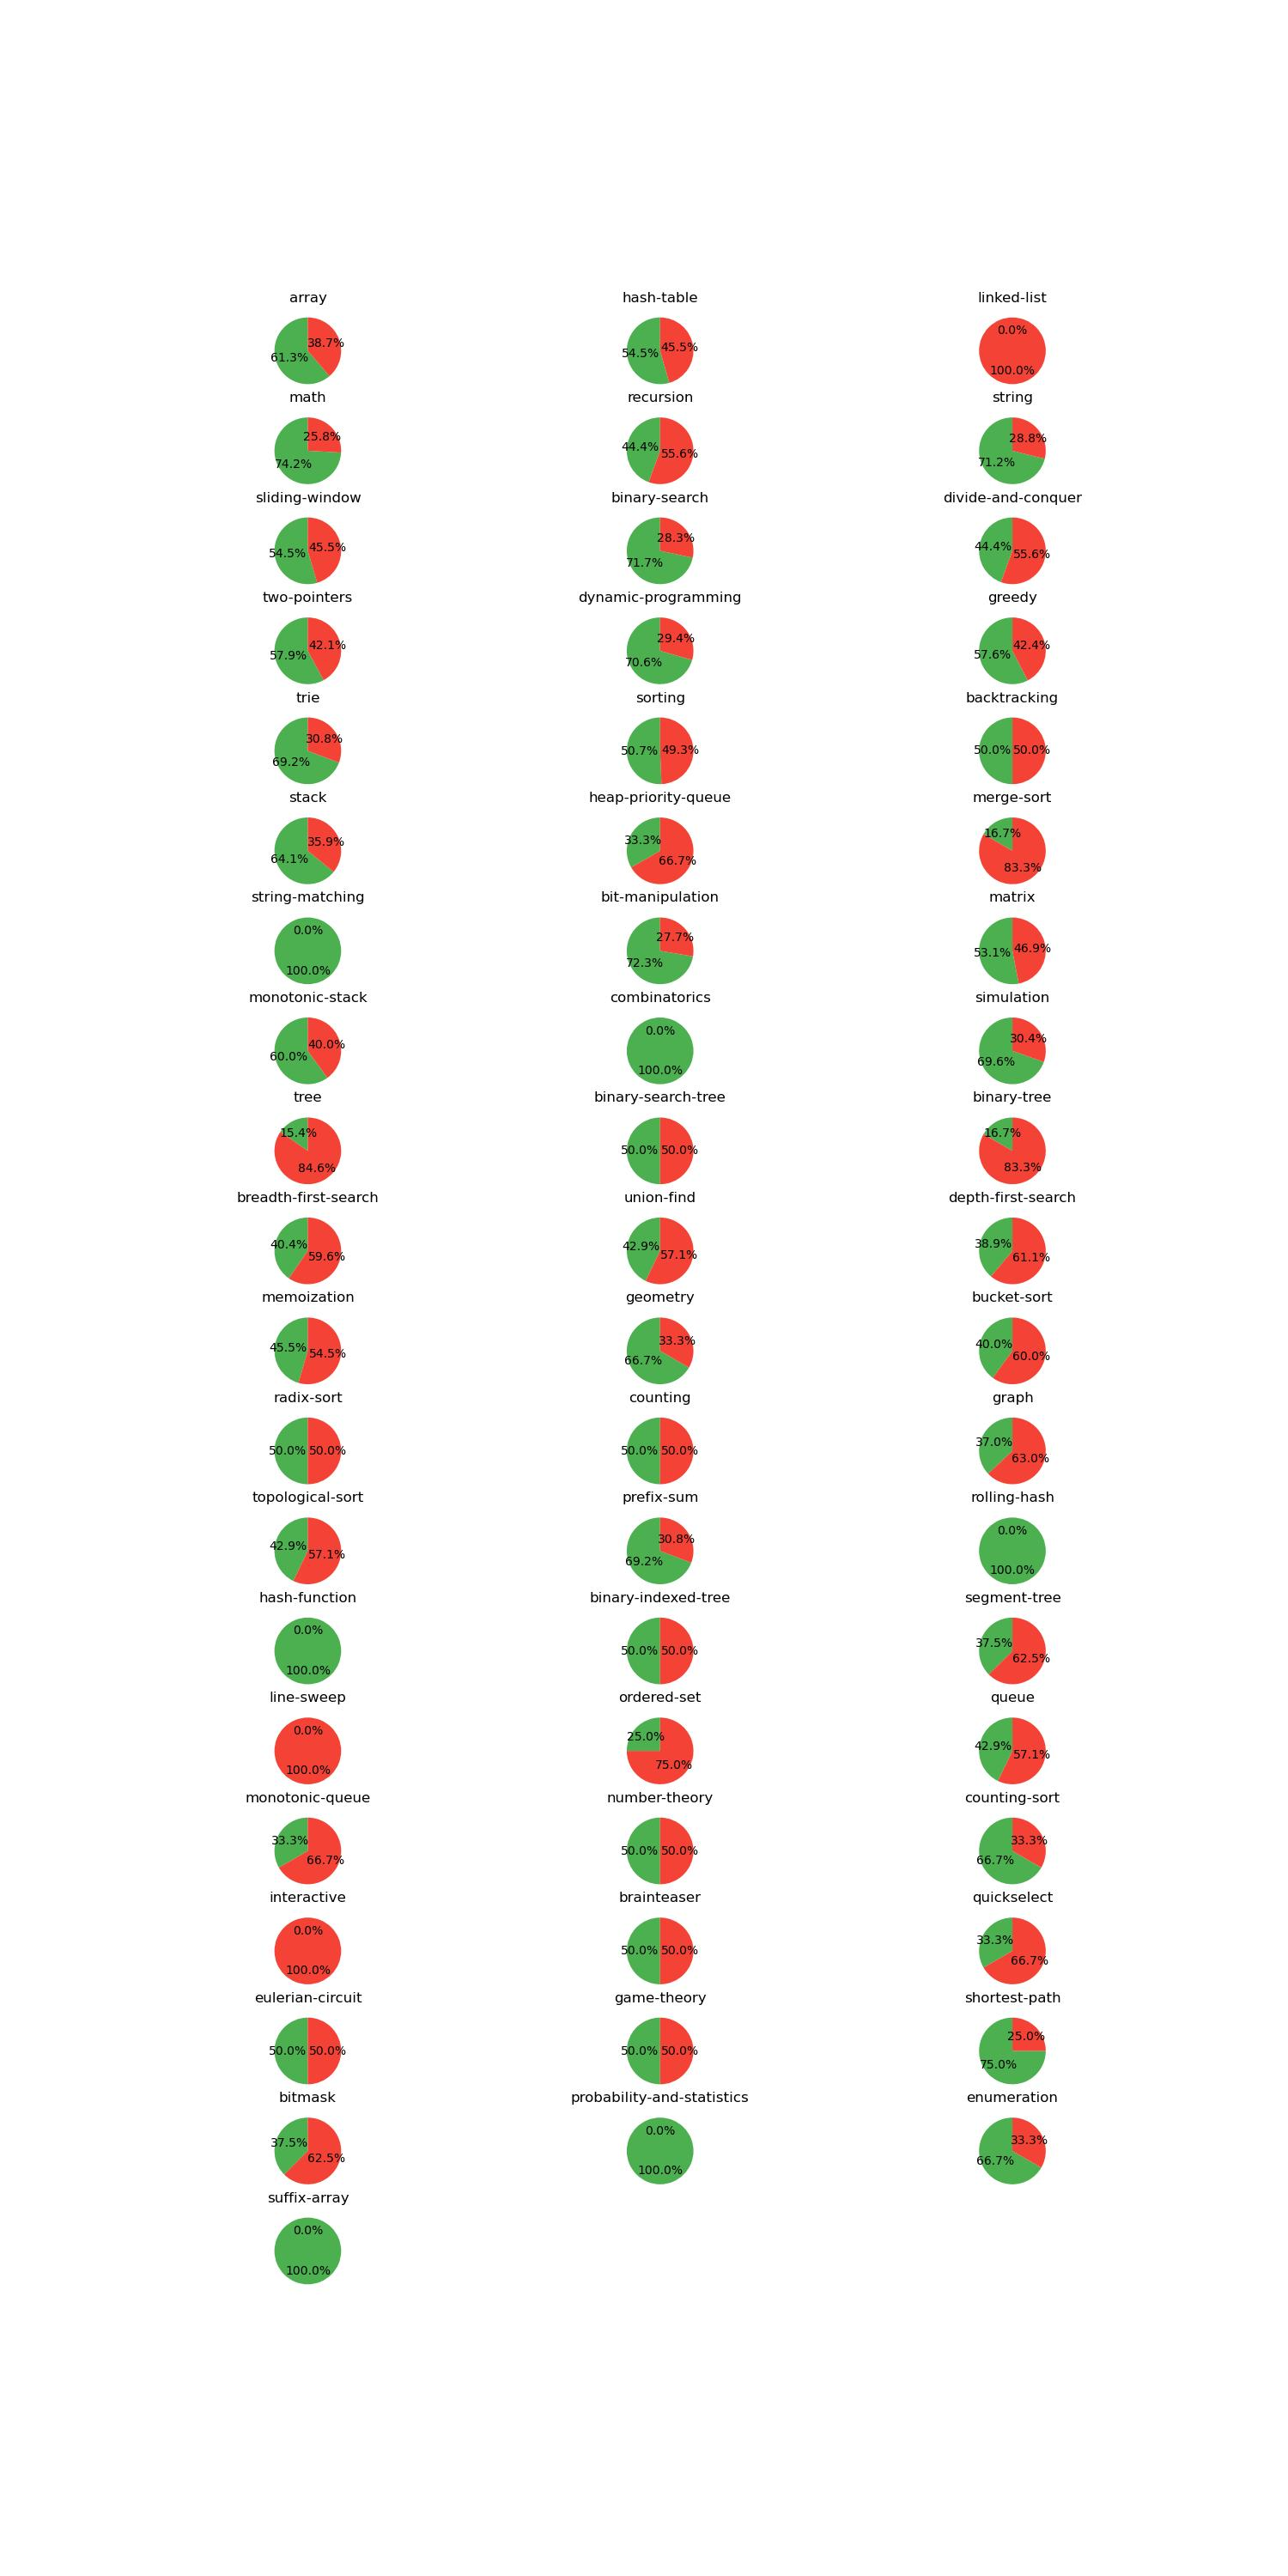
\includegraphics[width=0.75\textwidth, height=0.7\textheight]{figures/6/accepted_not_topicwise.jpg}
    \caption{Topic-wise acceptance rate for Prompt 6, illustrating the percentage of solutions accepted (green) and not accepted (red) across different undergraduate computer science topics.}
    \label{fig:topic_wise_acceptance_prompt_6}
\end{figure}

\begin{figure}[H]
    \centering
    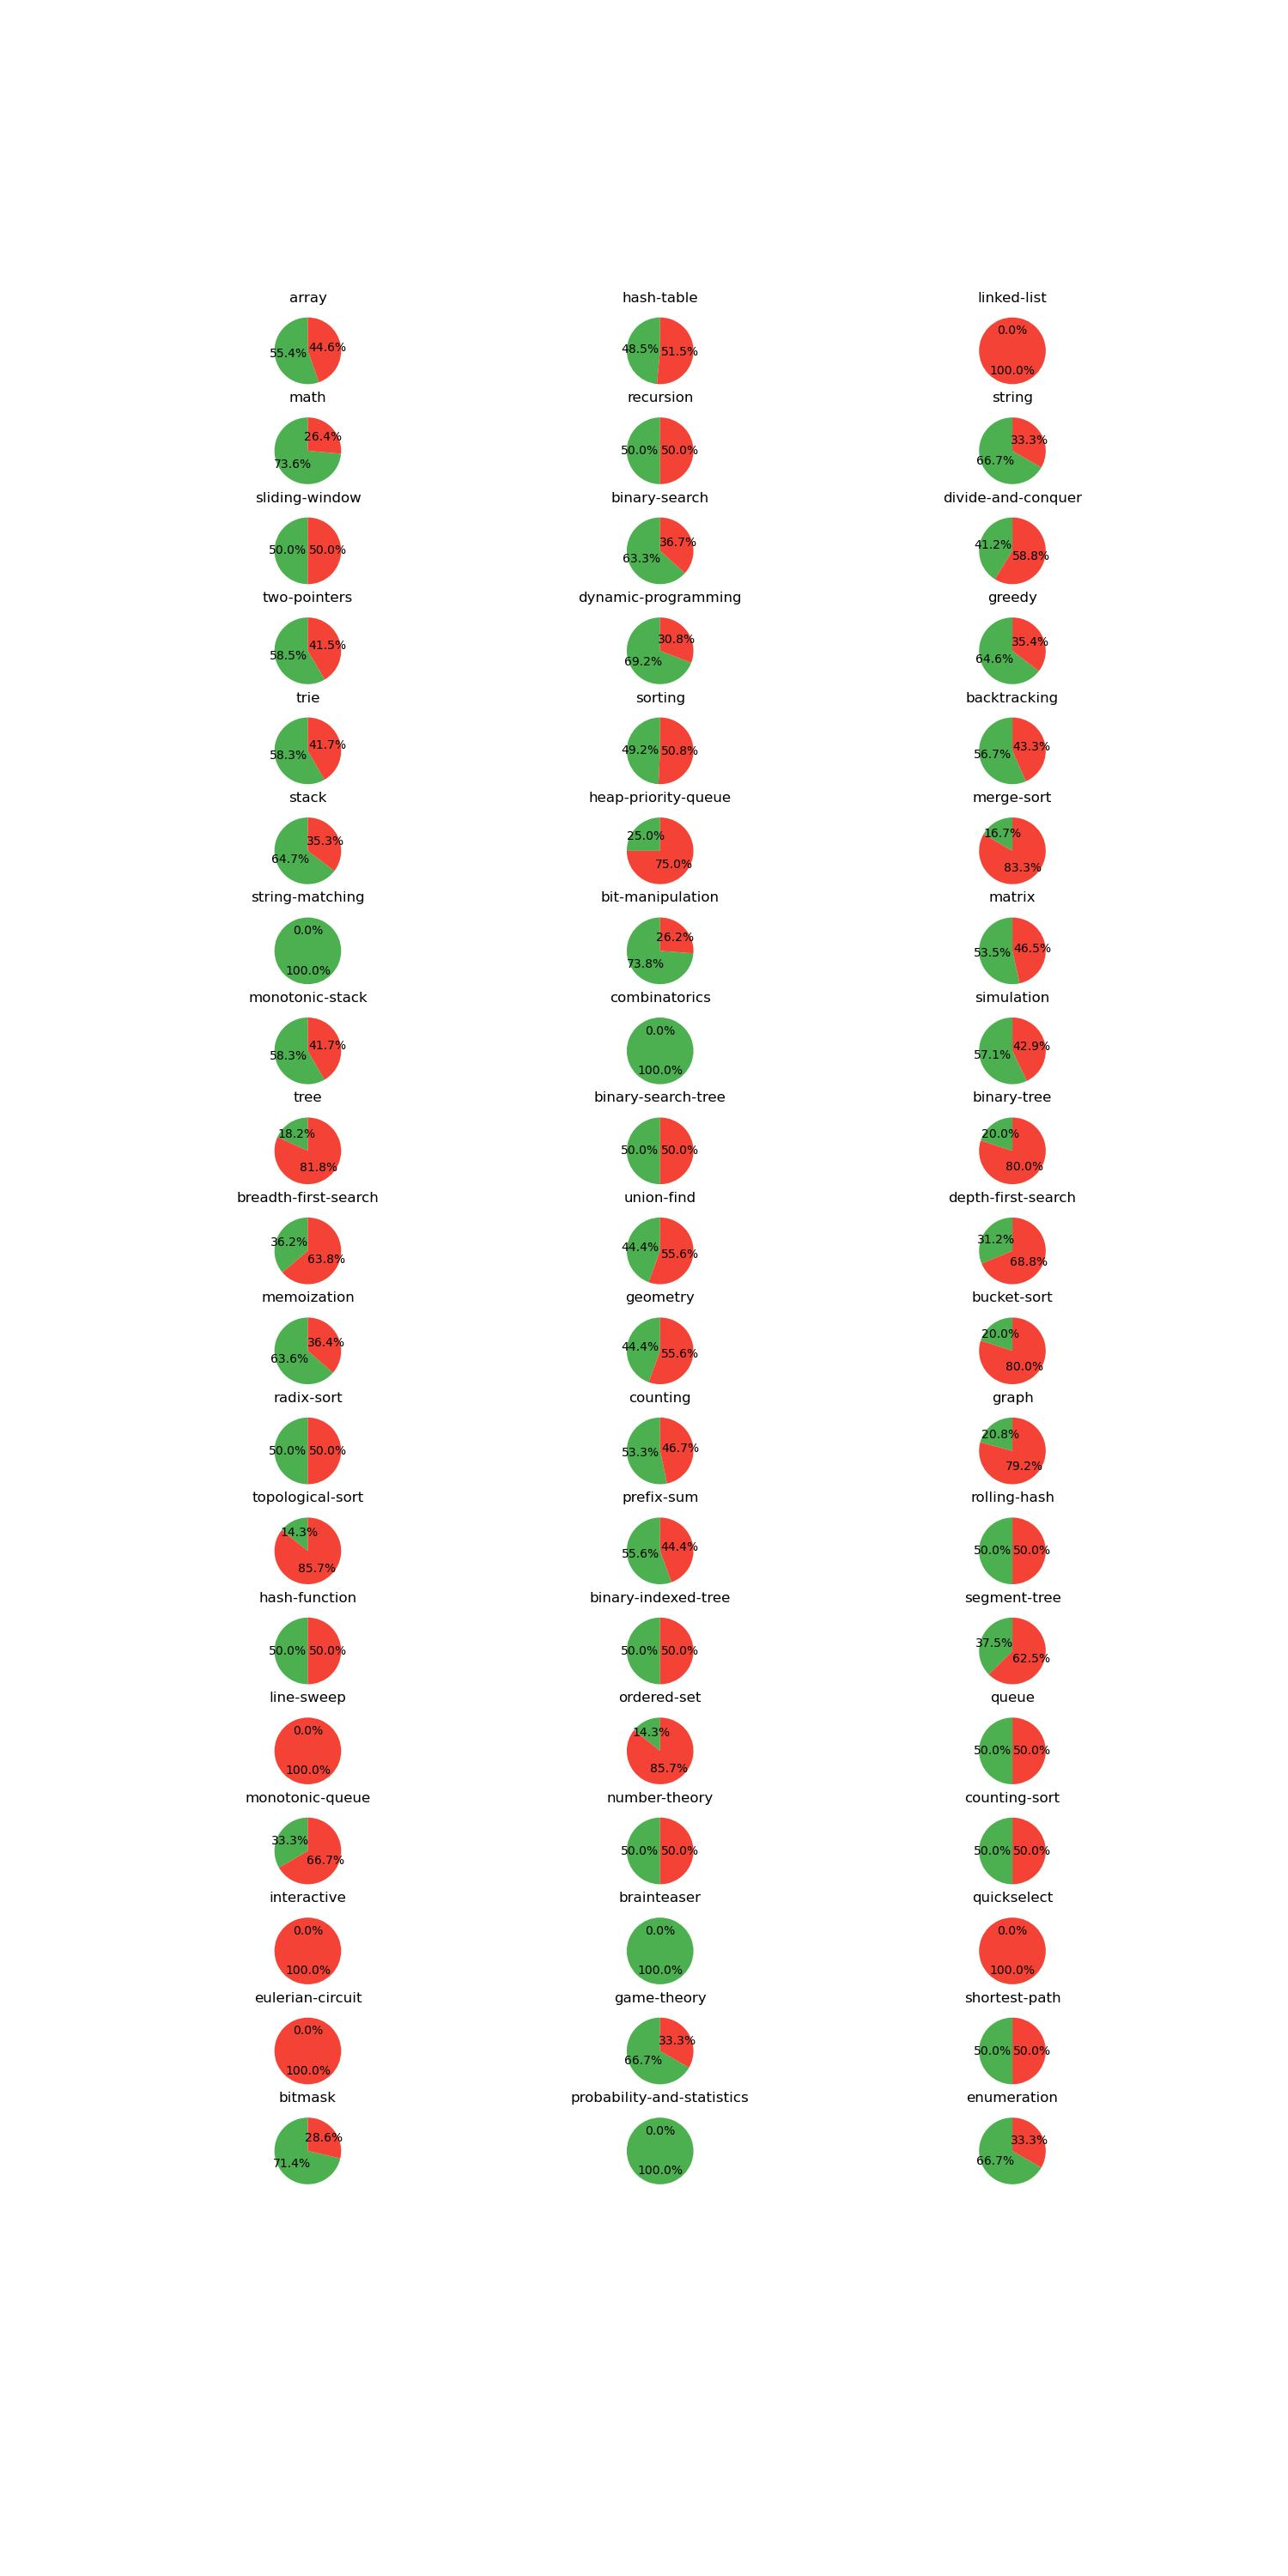
\includegraphics[width=0.75\textwidth, height=0.7\textheight]{figures/7/accepted_not_topicwise.jpg}
    \caption{Topic-wise acceptance rate for Prompt 7, illustrating the percentage of solutions accepted (green) and not accepted (red) across different undergraduate computer science topics.}
    \label{fig:topic_wise_acceptance_prompt_7}
\end{figure}

\begin{figure}[H]
    \centering
    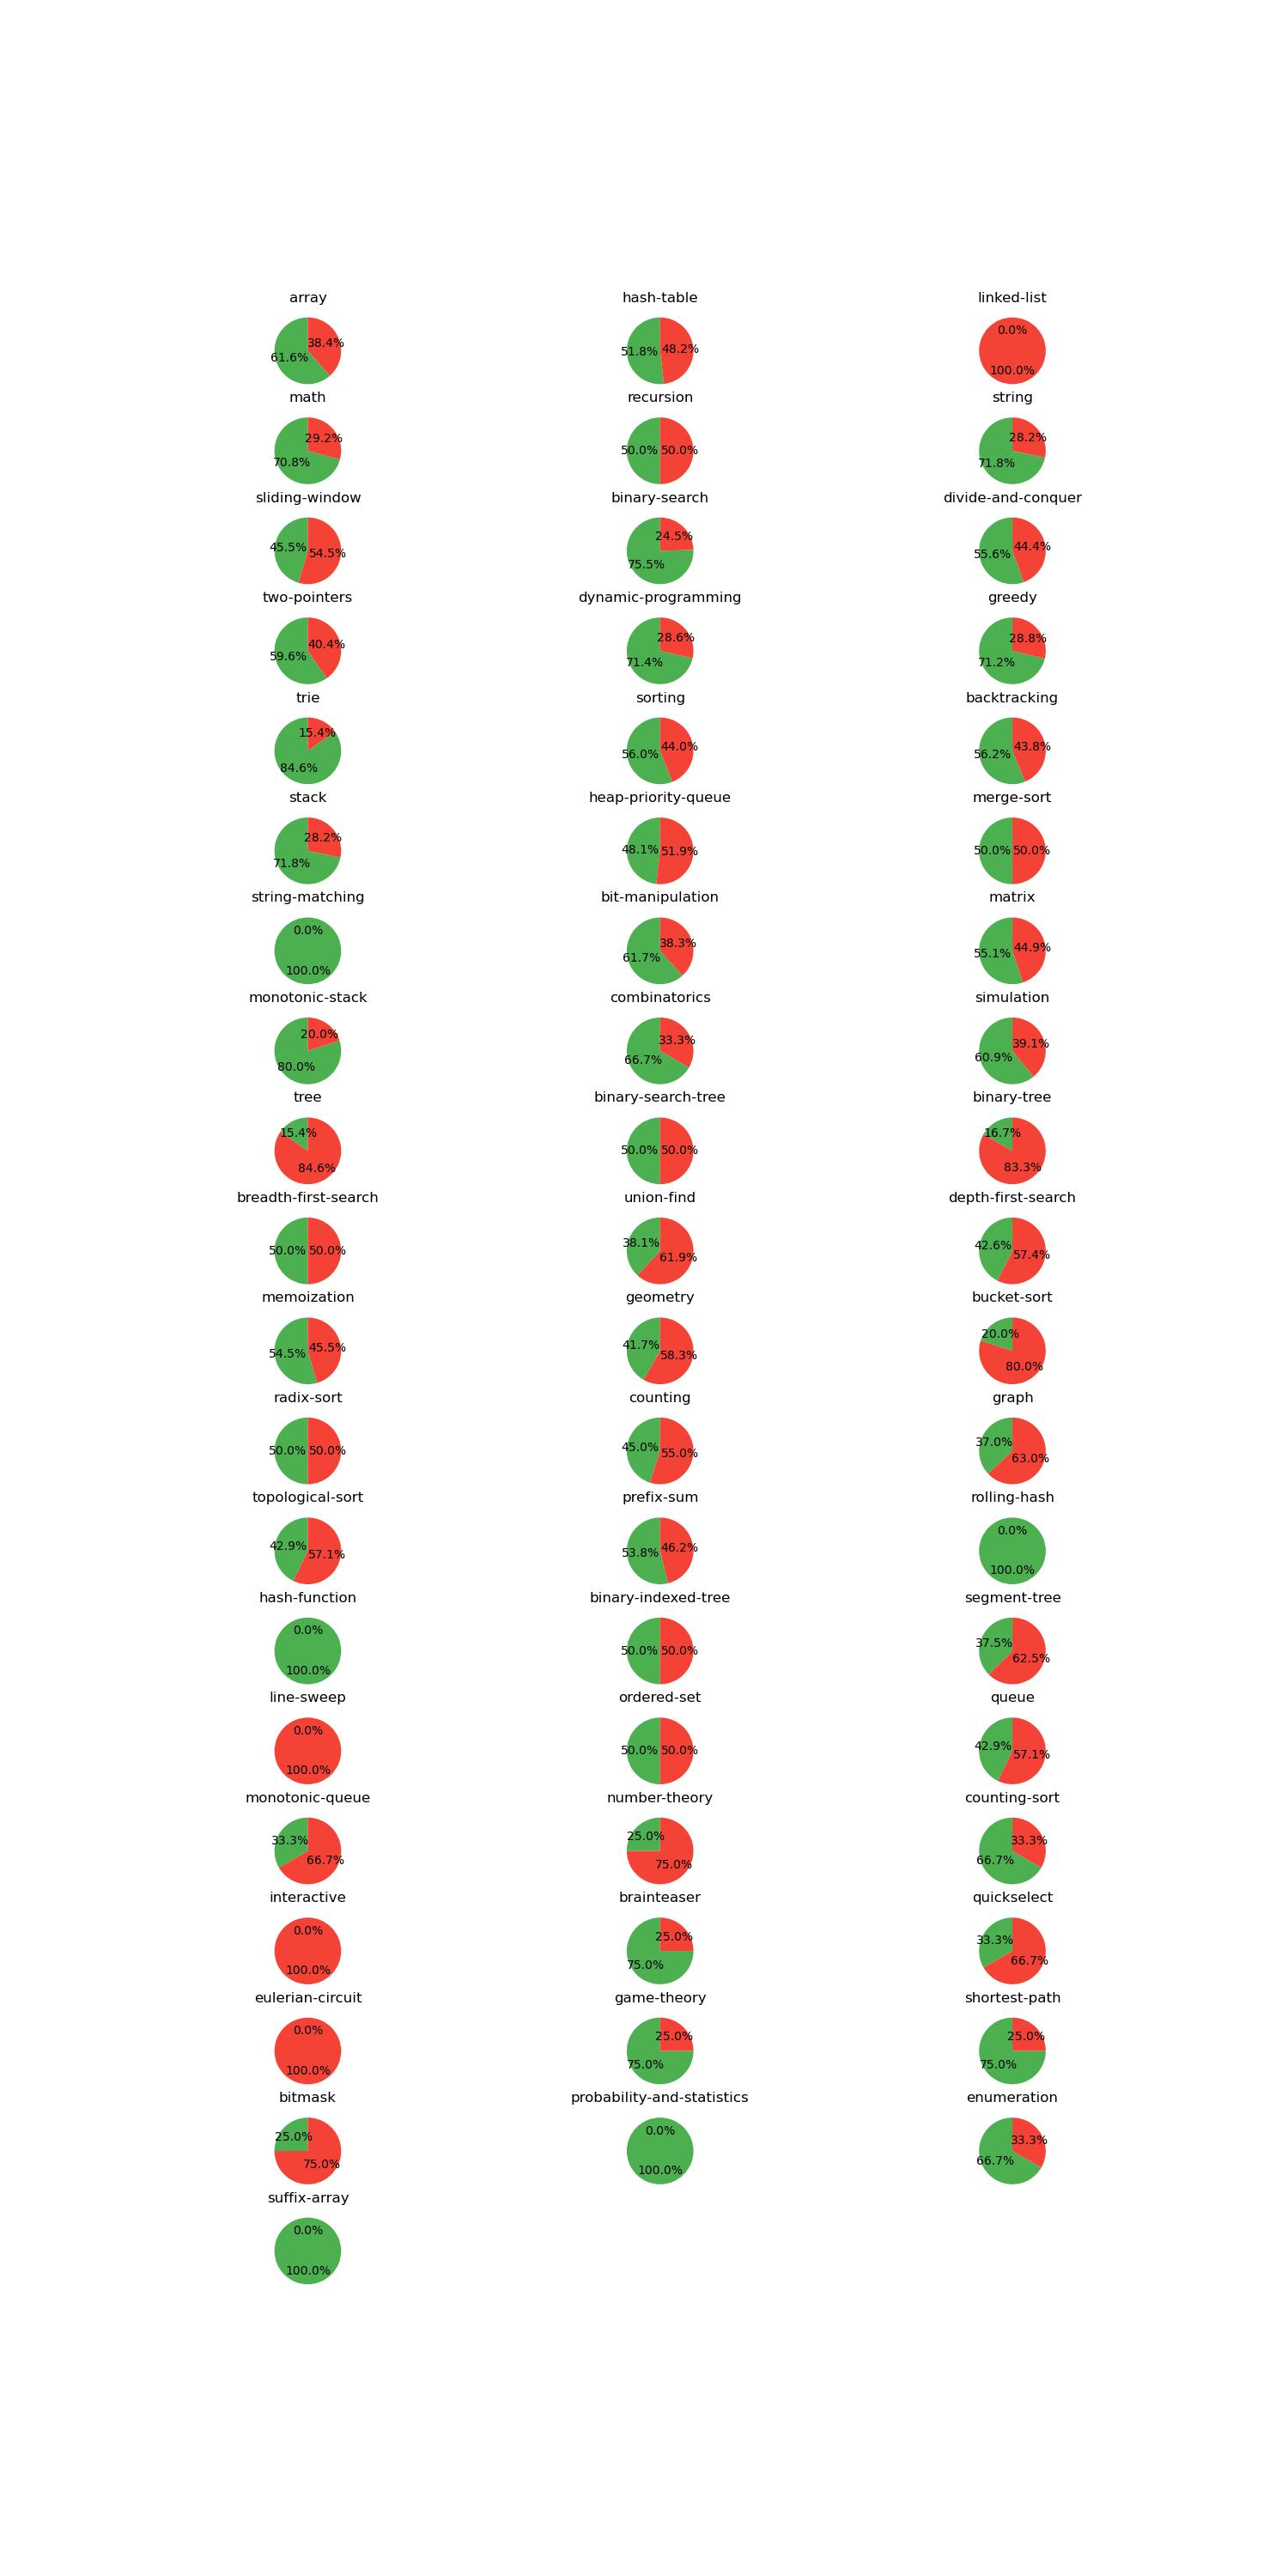
\includegraphics[width=0.75\textwidth, height=0.7\textheight]{figures/8/accepted_not_topicwise.jpg}
    \caption{Topic-wise acceptance rate for Prompt 8, illustrating the percentage of solutions accepted (green) and not accepted (red) across different undergraduate computer science topics.}
    \label{fig:topic_wise_acceptance_prompt_8}
\end{figure}

\begin{figure}[H]
    \centering
    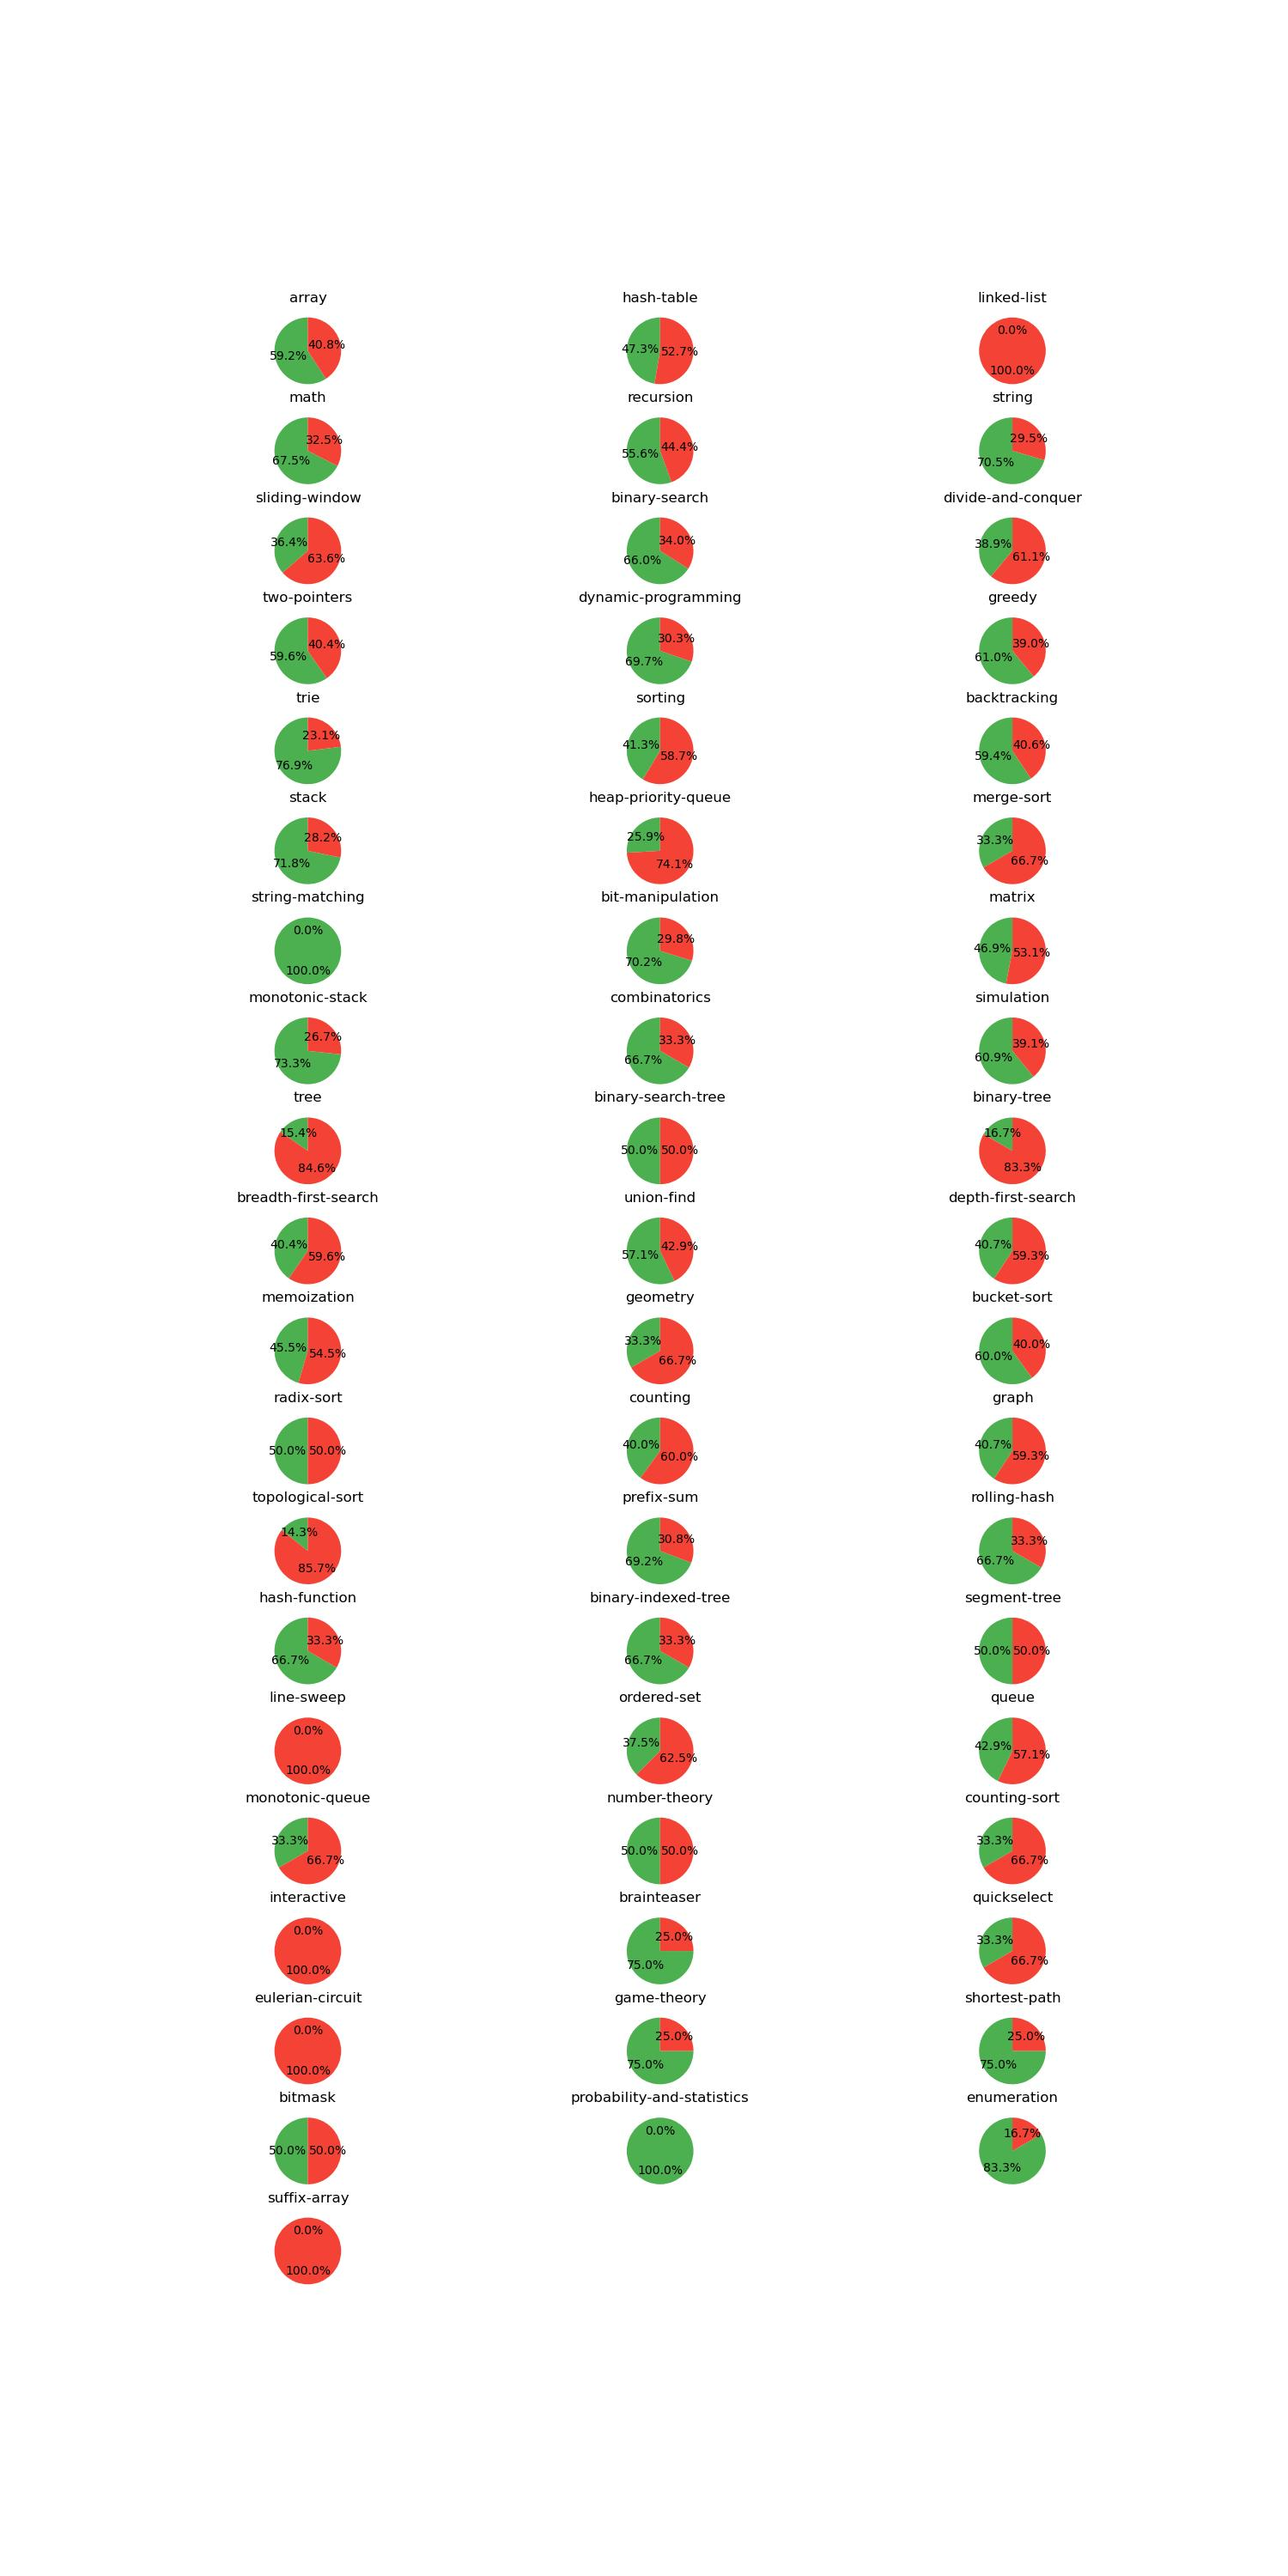
\includegraphics[width=0.75\textwidth, height=0.7\textheight]{figures/9/accepted_not_topicwise.jpg}
    \caption{Topic-wise acceptance rate for Prompt 9, illustrating the percentage of solutions accepted (green) and not accepted (red) across different undergraduate computer science topics.}
    \label{fig:topic_wise_acceptance_prompt_9}
\end{figure}
